% ============================================================
%  يُترجَم بـ XeLaTeX  (في Overleaf: Menu → Compiler → XeLaTeX)
%  الخط: Amiri (متوفر في Overleaf، أو حمّله من github.com/aliftype/amiri)
% ============================================================
\documentclass[12pt,a4paper]{article}
\usepackage[a4paper,margin=1.7cm,top=2.3cm,bottom=2.9cm,headheight=15pt,footskip=1.5cm]{geometry}
\usepackage{amsmath,amssymb}
\usepackage{icomma}
\usepackage[english,bidi=default,layout=lists]{babel}
\babelprovide[import,main]{arabic}
\babelfont{rm}[Scale=1.08]{Amiri}
\babelfont{sf}[Scale=1.08]{Amiri}
\usepackage[most]{tcolorbox}
\usepackage{tikz}
\usetikzlibrary{arrows.meta,calc,shadings}
\usepackage{array}
\usepackage{colortbl}
\usepackage{fancyhdr}
\usepackage{titlesec}
\usepackage{enumitem}
\usepackage{collcell}
\usepackage{needspace}
\usepackage{etoolbox}
\newcolumntype{C}{>{\collectcell\ar}c<{\endcollectcell}}
\pretocmd{\section}{\Needspace{15\baselineskip}}{}{}
\pretocmd{\subsection}{\Needspace{11\baselineskip}}{}{}

\definecolor{cDef}{HTML}{1F4E9C}
\definecolor{cThm}{HTML}{B3261E}
\definecolor{cRem}{HTML}{2E7D32}
\definecolor{cEx}{HTML}{C76B00}
\definecolor{cMeth}{HTML}{6A1B9A}
\definecolor{cSol}{HTML}{00695C}
\definecolor{cSec}{HTML}{1F3A68}

\titleformat{\section}{\Large\bfseries\color{cSec}}{\thesection.}{0.6em}{}[{\color{cSec!60}\titlerule[1pt]}]
\titleformat{\subsection}{\large\bfseries\color{cThm!85!black}}{\thesubsection.}{0.5em}{}
\titlespacing*{\section}{0pt}{14pt}{8pt}
\titlespacing*{\subsection}{0pt}{10pt}{5pt}
\setlength{\parindent}{0pt}
\setlength{\parskip}{4pt}
\setlist{itemsep=2pt,topsep=3pt}

\newtcolorbox{arbox}[3][]{enhanced,
  colback=#2!5,colframe=#2!80!black,arc=2mm,boxrule=0.8pt,
  left=6pt,right=6pt,top=8pt,bottom=5pt,
  fonttitle=\bfseries,coltitle=white,
  title={\foreignlanguage{arabic}{#3}},
  attach boxed title to top right={xshift=-5mm,yshift=-3mm},
  boxed title style={colback=#2!80!black,arc=1.5mm,boxrule=0pt},
  before upper={\selectlanguage{arabic}},
  before skip=8pt,after skip=8pt,breakable,#1}
\newenvironment{BOX}[2]{\begin{otherlanguage}{english}\begin{arbox}{#1}{#2}}{\end{arbox}\end{otherlanguage}}
\newenvironment{tarif}[1][تعريف]{\begin{BOX}{cDef}{#1}}{\end{BOX}}
\newenvironment{khassia}[1][خاصية]{\begin{BOX}{cThm}{#1}}{\end{BOX}}
\newenvironment{molahada}[1][ملاحظة]{\begin{BOX}{cRem}{#1}}{\end{BOX}}
\newenvironment{mithal}[1][مثال]{\begin{BOX}{cEx}{#1}}{\end{BOX}}
\newenvironment{tariqa}[1][طريقة]{\begin{BOX}{cMeth}{#1}}{\end{BOX}}

\newcounter{exo}
\newenvironment{tamrin}[1]{\stepcounter{exo}\begin{BOX}{cSec}{التمرين \theexo: #1}}{\end{BOX}}
\newenvironment{hal}{\Needspace{12\baselineskip}\begin{otherlanguage}{english}\begin{arbox}[breakable]{cSol}{حل التمرين \theexo}}{\end{arbox}\end{otherlanguage}}

\newenvironment{LTR}{\begin{otherlanguage}{english}}{\end{otherlanguage}}
\newcommand{\ar}[1]{\foreignlanguage{arabic}{#1}}

\renewcommand{\dots}{\mathinner{\ldotp\ldotp\ldotp}}
\renewcommand{\ldots}{\mathinner{\ldotp\ldotp\ldotp}}
\renewcommand{\cdots}{\mathinner{\cdotp\cdotp\cdotp}}
\newcommand{\N}{\mathbb{N}}
\newcommand{\Z}{\mathbb{Z}}
\newcommand{\D}{\mathbb{D}}
\newcommand{\Q}{\mathbb{Q}}
\newcommand{\R}{\mathbb{R}}
\newcommand{\pgcd}{\operatorname{PGCD}}
\newcommand{\ppcm}{\operatorname{PPCM}}

% \NLseg{a}{b}{[}{]} ; \NLright{a}{[} ; \NLleft{b}{]}  (interval on a number line)
\newcommand{\NLseg}[4]{\begin{LTR}\begin{tikzpicture}[baseline=-0.6ex]
 \draw[-{Stealth[length=2mm]},gray!70](0,0)--(3.4,0);
 \draw[line width=2pt,cThm!80!black](0.7,0)--(2.7,0);
 \node[cThm!80!black,font=\LARGE] at (0.7,0){$#3$};
 \node[cThm!80!black,font=\LARGE] at (2.7,0){$#4$};
 \node[below=3pt,font=\footnotesize] at (0.7,0){$#1$};
 \node[below=3pt,font=\footnotesize] at (2.7,0){$#2$};
\end{tikzpicture}\end{LTR}}
\newcommand{\NLright}[2]{\begin{LTR}\begin{tikzpicture}[baseline=-0.6ex]
 \draw[-{Stealth[length=2mm]},gray!70](0,0)--(3.4,0);
 \draw[line width=2pt,cThm!80!black](1.3,0)--(3.3,0);
 \node[cThm!80!black,font=\LARGE] at (1.3,0){$#2$};
 \node[below=3pt,font=\footnotesize] at (1.3,0){$#1$};
\end{tikzpicture}\end{LTR}}
\newcommand{\NLleft}[2]{\begin{LTR}\begin{tikzpicture}[baseline=-0.6ex]
 \draw[-{Stealth[length=2mm]},gray!70](0,0)--(3.4,0);
 \draw[line width=2pt,cThm!80!black](0.05,0)--(2.1,0);
 \node[cThm!80!black,font=\LARGE] at (2.1,0){$#2$};
 \node[below=3pt,font=\footnotesize] at (2.1,0){$#1$};
\end{tikzpicture}\end{LTR}}

% ---------- social-media icons (pure TikZ) ----------
\definecolor{cFB}{HTML}{1877F2}
\definecolor{cTG}{HTML}{229ED9}
\definecolor{cIG1}{HTML}{FEDA75}
\definecolor{cIG2}{HTML}{D62976}
\definecolor{cIG3}{HTML}{4F5BD5}
\newcommand{\fbicon}{\begin{LTR}\begin{tikzpicture}[baseline=-0.75ex,x=1em,y=1em]
 \fill[cFB] (0,0) circle (0.55);
 \node[white,inner sep=0,font=\usefont{TU}{lmss}{bx}{n}\small] at (0.04,-0.02) {f};
\end{tikzpicture}\end{LTR}}
\newcommand{\igicon}{\begin{LTR}
\begin{tikzpicture}[baseline=-0.75ex,x=1em,y=1em]
 \shade[lower left=cIG1,lower right=cIG2,upper left=cIG2,upper right=cIG3,rounded corners=0.28em] (-0.55,-0.55) rectangle (0.55,0.55);
 \draw[white,line width=0.09em,rounded corners=0.18em] (-0.36,-0.36) rectangle (0.36,0.36);
 \draw[white,line width=0.09em] (0,0) circle (0.17);
 \fill[white] (0.22,0.22) circle (0.05);
\end{tikzpicture}\end{LTR}}
\newcommand{\tgicon}{\begin{LTR}
\begin{tikzpicture}[baseline=-0.75ex,x=1em,y=1em]
 \fill[cTG] (0,0) circle (0.55);
 \fill[white] (-0.33,0.0) -- (0.32,0.27) -- (0.2,-0.3) -- (0.0,-0.15) -- (-0.08,-0.28) -- (-0.08,-0.08) -- cycle;
 \fill[cTG!70!black] (-0.08,-0.08) -- (0.25,0.2) -- (0.0,-0.15) -- (-0.08,-0.28) -- cycle;
\end{tikzpicture}\end{LTR}}
% page number: black box, white two-digit number, at the right of the social row
\newcommand{\PageBox}{\begin{LTR}\tikz[baseline=(p.base)]\node[fill=black,text=white,inner sep=2.5pt,minimum width=1.6em,minimum height=1.3em,font=\usefont{TU}{lmss}{bx}{n}\small](p){\ifnum\value{page}<10 0\fi\arabic{page}};\end{LTR}}
% visual left-to-right order: Telegram | Instagram | Facebook | page box
\newcommand{\SocialRow}{\begin{otherlanguage}{english}%
 \ar{\textbf{الأستاذ سوايسية هشام للرياضيات}}\ \tgicon\hfill
 \textbf{prof\_hicham\_math}\ \igicon\hfill
 \ar{\textbf{الأستاذ سوايسية هشام للرياضيات}}\ \fbicon\hspace{2.2em}\PageBox\end{otherlanguage}}

\pagestyle{fancy}
\fancyhf{}
\renewcommand{\headrulewidth}{0.6pt}
\renewcommand{\footrulewidth}{0.4pt}
% \SetHeader{right head: document title}{left head: level -- stream}
\newcommand{\SetHeader}[2]{%
 \fancyhead[C]{\parbox{\textwidth}{\ar{#1\hfill #2}}}%
 \fancyfoot[C]{\parbox{\textwidth}{\small\SocialRow}}}
\usepackage{tkz-tab}
\usepackage{multicol}
% variation / sign table (LTR)
\newenvironment{TAB}{\par\begin{center}\begin{LTR}\begin{tikzpicture}[scale=0.95,every node/.style={font=\small}]}{\end{tikzpicture}\end{LTR}\end{center}}
% grid + axes, clipped: \begin{GR}{xmin}{xmax}{ymin}{ymax}{unit cm}
\newenvironment{GR}[5]{\par\begin{center}\begin{LTR}\begin{tikzpicture}[x=#5cm,y=#5cm,font=\footnotesize]
 \draw[gray!25,very thin] (#1,#3) grid (#2,#4);
 \draw[-{Stealth[length=2mm]}] (#1,0)--(#2+0.3,0) node[below left]{$x$};
 \draw[-{Stealth[length=2mm]}] (0,#3)--(0,#4+0.3) node[below left]{$y$};
 \node[below left] at (0,0){$O$};
 \begin{scope}\clip (#1,#3) rectangle (#2,#4);}
{\end{scope}\end{tikzpicture}\end{LTR}\end{center}}
\newcommand{\Ticks}[2]{\foreach \t in {#1} \node[below,font=\scriptsize] at (\t,0){$\t$}; \foreach \t in {#2} \node[left,font=\scriptsize] at (0,\t){$\t$};}
\newcommand{\bx}[1]{\ensuremath{\colorbox{cDef!12}{$\displaystyle #1$}}}
\newcommand{\TwoCol}[4]{\par\begin{LTR}\noindent\begin{minipage}[t]{#1\textwidth}\selectlanguage{arabic}#2\end{minipage}\hfill\begin{minipage}[t]{#3\textwidth}\selectlanguage{arabic}#4\end{minipage}\end{LTR}\par}
\newcommand{\RL}[4]{\TwoCol{#3}{#4}{#1}{#2}}  % \RL{w1}{right content}{w2}{left content}
\newcommand{\ok}{$\textcolor{cRem}{\checkmark}$}
\newcommand{\limn}{\displaystyle\lim_{n\to+\infty}}
% sub-questions, each on its own line
\newenvironment{sq}{\begin{itemize}[leftmargin=2.4em,itemsep=3pt]}{\end{itemize}}
\newcommand{\qa}{\item[(أ)]}\newcommand{\qb}{\item[(ب)]}\newcommand{\qc}{\item[(جـ)]}\newcommand{\qd}{\item[(د)]}\newcommand{\qe}{\item[(هـ)]}
\newcommand{\pa}{\par\smallskip\textbf{(أ)} }\newcommand{\pb}{\par\smallskip\textbf{(ب)} }\newcommand{\pc}{\par\smallskip\textbf{(جـ)} }\newcommand{\pd}{\par\smallskip\textbf{(د)} }\newcommand{\pe}{\par\smallskip\textbf{(هـ)} }
\newcommand{\QQ}[1]{\par\smallskip\textbf{#1.} }
\newenvironment{tmr}{\stepcounter{exo}\begin{BOX}{cSec}{تمرين محلول \theexo}}{\end{BOX}}
\newcommand{\ABC}[3]{\\[2pt]\begin{tabular}{p{0.28\textwidth}p{0.28\textwidth}p{0.28\textwidth}}(جـ) \ #3 & (ب) \ #2 & (أ) \ #1\end{tabular}}
\pretocmd{\section}{\Needspace{24\baselineskip}}{}{}
\newtcbox{\bxtbox}{on line,colback=cDef!12,colframe=cDef!12,boxrule=0pt,arc=1pt,boxsep=0pt,left=2pt,right=2pt,top=1pt,bottom=1pt}
\newcommand{\bxt}[1]{\foreignlanguage{english}{\bxtbox{\ar{#1}}}}
\usepackage{longtable}
\setlength{\LTpre}{4pt}\setlength{\LTpost}{0pt}
\newcommand{\Phase}[1]{\textbf{#1}}
\newcommand{\Fld}[2]{\textbf{#1:}\ #2}
% رأس المذكرة على نمط النموذج: إطار بعنوان «مذكرة رقم»، معلومات الحصة، ثم إطار الكفاءات
\newcommand{\ModhHead}[9]{%
\begin{LTR}
\begin{tcolorbox}[enhanced,colback=white,colframe=cThm!85!black,arc=4mm,boxrule=1pt,top=14pt,bottom=6pt,left=8pt,right=8pt,
 overlay={\node[fill=cThm!85!black,text=white,rounded corners=3mm,inner xsep=14pt,inner ysep=4pt,font=\large\bfseries] at ([yshift=0pt]frame.north){\ar{مذكرة رقم #1}};},
 before upper={\selectlanguage{arabic}}]
\begin{tabular}{@{}p{0.4\linewidth}p{0.55\linewidth}@{}}
\Fld{المستوى}{#2} & \Fld{الثانوية}{\dotfill}\\[3pt]
\Fld{المادة}{رياضيات} & \Fld{ميدان التعلم}{#3}\\[3pt]
\Fld{المدة}{#5} & \Fld{الوحدة التعلمية}{#4}\\[3pt]
\Fld{الأستاذ}{\dotfill} & \Fld{المحتوى المعرفي}{#6}\\
\end{tabular}
\end{tcolorbox}
\begin{tcolorbox}[enhanced,colback=white,colframe=cThm!85!black,arc=3mm,boxrule=0.8pt,sidebyside,sidebyside align=top,lefthand ratio=0.5,
 segmentation style={dashed,cThm!60},before upper={\selectlanguage{arabic}},before lower={\selectlanguage{arabic}}]
\textbf{الكفاءات المستهدفة:}\par #8
\tcblower
\textbf{الكفاءات القبلية:}\par #7
\end{tcolorbox}
\end{LTR}
\par\smallskip\textbf{الوسائل:} #9\par\smallskip}
\newenvironment{Sayr}{%
\begin{LTR}\renewcommand{\arraystretch}{1.25}
\begin{longtable}{|p{0.17\textwidth}|>{\centering\arraybackslash}p{0.06\textwidth}|p{0.53\textwidth}|>{\centering\arraybackslash}p{0.12\textwidth}|}
\hline\rowcolor{cThm!12}\ar{\textbf{توجيهات وتعاليق}} & \ar{\textbf{المدة}} & \ar{\textbf{سير الحصة}} & \ar{\textbf{مراحل الحصة}}\\\hline\endhead
\hline\endfoot}{\end{longtable}\end{LTR}}
% سطر في الجدول: \Row{مرحلة}{سير}{مدة}{توجيهات}
\newcommand{\Row}[4]{\ar{\small #4} & \ar{#3} & \ar{#2} & \cellcolor{cThm!8}\ar{\Phase{#1}}\\\hline}

\newcommand{\Lab}[2]{\foreignlanguage{english}{\tcbox[on line,colback=#1,colframe=#1,boxrule=0pt,arc=2pt,boxsep=1pt,left=5pt,right=5pt,top=1pt,bottom=1pt]{\ar{\textcolor{white}{\textbf{#2}}}}}}
\newcommand{\Num}[1]{\foreignlanguage{english}{\tikz[baseline=(c.base)]\node[fill=cDef,text=white,inner sep=2pt,font=\footnotesize\bfseries](c){#1};}}
\newcommand{\ck}{\ensuremath{{\color{cRem}\checkmark}}}
\newenvironment{Kad}[1]{\par\smallskip\Lab{#1}}{\par}
\SetHeader{\small\bfseries\color{cSec}مذكرات محور: النهايات}{\small\color{cSec}السنة الثانية ثانوي -- علوم تجريبية}
\begin{document}
\begin{LTR}
\begin{tcolorbox}[enhanced,colback=cThm!85!black,colframe=cThm!85!black,arc=3mm,halign=center,boxrule=0pt,top=12pt,bottom=12pt,before upper={\selectlanguage{arabic}}]
{\color{white}\fontsize{26}{32}\selectfont\bfseries مذكرات محور: النهايات}\\[8pt]
{\color{white}\large السنة الثانية ثانوي -- علوم تجريبية (صالحة لشعبتي رياضيات وتقني رياضي)}\\[4pt]
{\color{white}\large 6 مذكرات (12 ساعة) -- السنة الدراسية 2026-2027}
\end{tcolorbox}
\end{LTR}
\begin{BOX}{cThm}{يتضمن هذا العمل}
\begin{enumerate}[label=\textbf{مذكرة \arabic{enumi}:},leftmargin=6em,start=31]
\item نهاية دالة عند $+\infty$ و $-\infty$ ، المقارب الأفقي.
\item نهاية غير منتهية عند عدد حقيقي ، المقارب العمودي.
\item العمليات على النهايات.
\item إزالة حالة عدم التعيين.
\item المستقيم المقارب المائل.
\item دراسة دالة ناطقة وتمثيلها البياني.
\end{enumerate}
مراجع النشاطات والتمارين: الكتاب المدرسي للسنة الثانية ثانوي (باب النهايات ص 110--111). شعبة رياضيات: يضاف «البحث عن» المقارب المائل.
\end{BOX}
\newpage
\ModhHead{31}{2 ع ت}{تحليل}{النهايات}{02 سا}{نهاية دالة عند $+\infty$ و $-\infty$ ، المستقيم المقارب الموازي لمحور الفواصل}%
{\begin{itemize}\item الدوال المرجعية ، جدول التغيرات.\end{itemize}}%
{\begin{itemize}\item حساب نهاية دالة عند $\pm\infty$.\item التعرف على مستقيم مقارب أفقي.\end{itemize}}%
{المنهاج ، الكتاب المدرسي ، مراجع ، الحاسبة البيانية.}
\begin{Sayr}
\Row{مرحلة الانطلاق}{%
\textbf{التهيئة النفسية:} ماذا يحدث للعدد $\dfrac1x$ لما يكبر $x$ كثيراً؟ ($x=10$ ، $1000$ ، $10^6$)}{10 د}{سؤال بالحاسبة.}
\Row{التشخيص والاكتشاف}{%
\Lab{cEx}{مناقشة النشاطين 03 صفحة 110 و 04 صفحة 111}\par\ck\ الدالة مربع: لما يأخذ $x$ قيماً كبيرة جداً يصبح $x^2$ أكبر من أي عدد نختاره.\par
\ck\ دالة ناطقة: جداول قيم لما $x$ كبير جداً ، القيم تقترب من عدد ثابت ، والمنحني يقترب من مستقيم أفقي.\par
}{35 د}{جداول قيم.}
\Row{بناء المعارف}{%
\Lab{cDef}{تعريف}\par\ck\ $\lim\limits_{x\to +\infty}f(x)=+\infty$: $f(x)$ يصبح أكبر من أي عدد لما يكبر $x$ بالقدر الكافي.\par
\ck\ $\lim\limits_{x\to +\infty}f(x)=l$: $f(x)$ يقترب من $l$ بالقدر الذي نريد ؛ نقول إن المستقيم $y=l$ \textbf{مقارب} لـ $C_f$ بجوار $+\infty$.\par
\Lab{cThm}{نهايات مرجعية}\ $\lim\limits_{x\to +\infty}x^2=+\infty$ ، $\lim\limits_{x\to -\infty}x^3=-\infty$ ، $\lim\limits_{x\to +\infty}\sqrt x=+\infty$ ، $\lim\limits_{x\to \pm\infty}\dfrac1x=0$ ، $\lim\limits_{x\to \pm\infty}\dfrac1{x^2}=0$.\par}{50 د}{نرسم المقارب بالمتقطع.}
\Row{}{%
\Lab{cEx}{مثال}\ $f(x)=3+\dfrac1x$: $\lim\limits_{x\to \pm\infty}f(x)=3$ ، المستقيم $y=3$ مقارب أفقي لـ $C_f$.\par\Lab{cThm!80!black}{حذار}\ $+\infty$ ليس عدداً حقيقياً: لا نعوض به في العبارة.}{}{}
\Row{التقويم}{%
\Lab{cEx}{تطبيق}\par احسب: $\lim\limits_{x\to +\infty}\left(5-\dfrac2{x^2}\right)$ ؛ $\lim\limits_{x\to +\infty}(x^2+\sqrt x)$ ؛ ثم استنتج مقارباً لمنحني $g(x)=2+\dfrac3{x-1}$.\par\textbf{الحل:} $5$ ؛ $+\infty$ ؛ $\lim\limits_{x\to \pm\infty}g(x)=2$ ، إذن $y=2$ مقارب أفقي.\par\textbf{واجب منزلي:} تمارين 15 ، 19 ، 20 ، 21 من باب النهايات.\par\smallskip\textbf{ملاحظات حول سير الحصة:} \dotfill}{25 د}{تقويم فردي.}
\end{Sayr}
\newpage
\ModhHead{32}{2 ع ت}{تحليل}{النهايات}{02 سا}{نهاية غير منتهية عند عدد حقيقي ، المستقيم المقارب الموازي لمحور التراتيب}%
{\begin{itemize}\item نهاية عند $\pm\infty$.\end{itemize}}%
{\begin{itemize}\item حساب نهاية دالة عند حد لمجموعة تعريفها.\item التفسير البياني لنهاية غير منتهية: المقارب العمودي.\end{itemize}}%
{المنهاج ، الكتاب المدرسي ، مراجع ، الحاسبة البيانية.}
\begin{Sayr}
\Row{مرحلة الانطلاق}{%
\textbf{التهيئة النفسية:} احسب $\dfrac1{x-1}$ من أجل $x=1{,}1$ ، $1{,}01$ ، $1{,}001$: ماذا تلاحظ؟ وإذا كان $x=0{,}999$ ؟}{10 د}{سؤال بالحاسبة.}
\Row{التشخيص والاكتشاف}{%
\Lab{cEx}{مناقشة النشاطين 01 و 02 صفحة 110}\par\ck\ جداول قيم لما يقترب $x$ من عدد $a$ من اليمين ومن اليسار.\par
\ck\ القيم تكبر (بالقيمة المطلقة) بلا حدود: نهاية غير منتهية ، وإشارتها تتعلق بالجهة.\par
}{35 د}{جداول اليمين واليسار.}
\Row{بناء المعارف}{%
\Lab{cDef}{تعريف}\ $\lim\limits_{x\to a}f(x)=+\infty$: $f(x)$ يصبح أكبر من أي عدد لما يقترب $x$ من $a$ بالقدر الكافي ؛ نميز النهاية \textbf{من اليمين} $x\to a^{+}$ و\textbf{من اليسار} $x\to a^{-}$.\par\Lab{cThm}{التفسير البياني}\ إذا كانت $\lim\limits_{x\to a}f(x)=\pm\infty$ (من جهة على الأقل) فإن المستقيم $x=a$ \textbf{مقارب عمودي} لـ $C_f$.\par}{50 د}{جدول إشارة المقام.}
\Row{}{%
\Lab{cEx}{مثال}\ $f(x)=\dfrac1{x-1}$: $\lim\limits_{x\to 1^{+}}f(x)=+\infty$ (المقام يؤول إلى $0^{+}$) و $\lim\limits_{x\to 1^{-}}f(x)=-\infty$ ؛ المستقيم $x=1$ مقارب عمودي.\par\Lab{cMeth}{طريقة}\ البسط يؤول إلى عدد غير معدوم والمقام إلى $0$: ندرس إشارة المقام بجوار $a$ في جدول.\par}{}{}
\Row{}{%
\Lab{cThm!80!black}{حذار}\ نكتب $0^{+}$ أو $0^{-}$ لتحديد إشارة النهاية.}{}{}
\Row{التقويم}{%
\Lab{cEx}{تطبيق}\par $g(x)=\dfrac{-2}{(x+3)^2}$. احسب نهاية $g$ عند $-3$ وفسّر بيانياً.\par\textbf{الحل:} $(x+3)^2\to0^{+}$ من الجهتين ، إذن $\lim\limits_{x\to -3}g(x)=-\infty$ ؛ المستقيم $x=-3$ مقارب عمودي.\par\textbf{واجب منزلي:} تمارين 14 ، 16 ، 18 ، 26 من باب النهايات.\par\smallskip\textbf{ملاحظات حول سير الحصة:} \dotfill}{25 د}{تقويم فردي.}
\end{Sayr}
\newpage
\ModhHead{33}{2 ع ت}{تحليل}{النهايات}{02 سا}{العمليات على النهايات}%
{\begin{itemize}\item النهايات المرجعية.\end{itemize}}%
{\begin{itemize}\item حساب نهايات باستعمال مبرهنات المجموع والجداء والمقلوب والقسمة.\item التعرف على حالات عدم التعيين.\end{itemize}}%
{المنهاج ، الكتاب المدرسي ، مراجع ، الحاسبة البيانية.}
\begin{Sayr}
\Row{مرحلة الانطلاق}{%
\textbf{التهيئة النفسية:} إذا كان $f(x)\to+\infty$ و $g(x)\to+\infty$ ، فإلى أين يؤول $f(x)-g(x)$ ؟ جرّب $x^2-x$ و $x-x^2$.}{10 د}{تحدٍّ.}
\Row{التشخيص والاكتشاف}{%
\Lab{cEx}{وضعية مقترحة}\par\ck\ $\lim\limits_{x\to +\infty}(x^2-x)=+\infty$ ، $\lim\limits_{x\to +\infty}(x-x^2)=-\infty$ ، $\lim\limits_{x\to +\infty}\big((x+1)-x\big)=1$.\par
\ck\ نفس الشكل «$+\infty-\infty$» يعطي نتائج مختلفة: \textbf{حالة عدم تعيين}.\par
}{35 د}{أمثلة مضادة.}
\Row{بناء المعارف}{%
\Lab{cThm}{نهاية المجموع}\par\smallskip\begin{LTR}\centering {\footnotesize\renewcommand{\arraystretch}{1.45}\begin{tabular}{|c|c|c|c|c|c|}\hline\rowcolor{cSec!12}$\lim f$ & $l$ & $l$ & $+\infty$ & $-\infty$ & $+\infty$\\\hline$\lim g$ & $l^{\prime}$ & $\pm\infty$ & $+\infty$ & $-\infty$ & $-\infty$\\\hline$\lim(f+g)$ & $l+l^{\prime}$ & $\pm\infty$ & $+\infty$ & $-\infty$ & \ar{ح ع ت}\\\hline\end{tabular}}\end{LTR}\par \Lab{cThm}{نهاية الجداء}\ (إشارة النتيجة بقاعدة الإشارات)\par\smallskip\begin{LTR}\centering {\footnotesize\renewcommand{\arraystretch}{1.45}\begin{tabular}{|c|c|c|c|c|}\hline\rowcolor{cSec!12}$\lim f$ & $l$ & $l\neq0$ & $\infty$ & $0$\\\hline$\lim g$ & $l^{\prime}$ & $\infty$ & $\infty$ & $\infty$\\\hline$\lim(f\times g)$ & $l\,l^{\prime}$ & $\infty$ & $\infty$ & \ar{ح ع ت}\\\hline\end{tabular}}\end{LTR}\par }{50 د}{الجداول تُنقل في الكراس.}
\Row{}{%
\Lab{cThm}{نهاية حاصل القسمة}\par\smallskip\begin{LTR}\centering {\footnotesize\renewcommand{\arraystretch}{1.45}\begin{tabular}{|c|c|c|c|c|c|c|}\hline\rowcolor{cSec!12}$\lim f$ & $l$ & $l$ & $l\neq0$ & $\infty$ & $\infty$ & $0$\\\hline$\lim g$ & $l^{\prime}\neq0$ & $\infty$ & $0$ & $l^{\prime}$ & $\infty$ & $0$\\\hline$\lim\dfrac fg$ & $\dfrac l{l^{\prime}}$ & $0$ & $\infty$ & $\infty$ & \ar{ح ع ت} & \ar{ح ع ت}\\\hline\end{tabular}}\end{LTR}\par \Lab{cRem}{ملاحظات}\ حالات عدم التعيين الأربع: $\infty-\infty$ ، $0\times\infty$ ، $\dfrac\infty\infty$ ، $\dfrac00$.}{}{}
\Row{التقويم}{%
\Lab{cEx}{تطبيق}\par احسب: $\lim\limits_{x\to +\infty}(x+1)\sqrt x$ ؛ $\lim\limits_{x\to -\infty}\dfrac1{x^2+1}$ ؛ $\lim\limits_{x\to 2^{+}}\dfrac{x+1}{x-2}$.\par\textbf{الحل:} $+\infty$ ؛ $0$ ؛ $+\infty$ (لأن $\dfrac3{0^{+}}$).\par\textbf{واجب منزلي:} تمارين 24 إلى 29 من باب النهايات.\par\smallskip\textbf{ملاحظات حول سير الحصة:} \dotfill}{25 د}{تقويم فردي.}
\end{Sayr}
\newpage
\ModhHead{34}{2 ع ت}{تحليل}{النهايات}{02 سا}{إزالة حالة عدم التعيين}%
{\begin{itemize}\item العمليات على النهايات ، التحليل.\end{itemize}}%
{\begin{itemize}\item إزالة حالات عدم التعيين لدوال كثيرات حدود وناطقة وصماء بسيطة.\end{itemize}}%
{المنهاج ، الكتاب المدرسي ، مراجع ، الحاسبة البيانية.}
\begin{Sayr}
\Row{مرحلة الانطلاق}{%
\textbf{التهيئة النفسية:} $\lim\limits_{x\to +\infty}(x^2-5x)$: لماذا لا نستطيع الحساب مباشرة؟}{10 د}{سؤال تشخيصي.}
\Row{التشخيص والاكتشاف}{%
\Lab{cEx}{وضعية مقترحة}\par\ck\ $x^2-5x=x^2\left(1-\dfrac5x\right)$: الجداء $+\infty\times1$ ، النهاية $+\infty$.\par
\ck\ نستنتج أن الحد الأعلى درجة هو الذي «يتحكم» عند المالانهاية.\par
}{35 د}{التحليل بالعامل المشترك.}
\Row{بناء المعارف}{%
\Lab{cThm}{عند $\pm\infty$}\par\ck\ نهاية كثير حدود هي نهاية حده الأعلى درجة.\par
\ck\ نهاية دالة ناطقة هي نهاية حاصل قسمة الحدين الأعليين درجة.\par
\Lab{cEx}{مثال}\ $\lim\limits_{x\to +\infty}\dfrac{2x^2+x}{x^2-3}=\lim\limits_{x\to +\infty}\dfrac{2x^2}{x^2}=2$.\par}{50 د}{نقارن الطرق.}
\Row{}{%
\Lab{cMeth}{حالة $\frac00$ عند عدد}\ نحلل ونختزل ، أو نضرب في المرافق.\par\ck\ $\lim\limits_{x\to 2}\dfrac{x^2-4}{x-2}=\lim\limits_{x\to 2}(x+2)=4$.\par
\ck\ $\lim\limits_{x\to 1}\dfrac{\sqrt x-1}{x-1}=\lim\limits_{x\to 1}\dfrac1{\sqrt x+1}=\dfrac12$.\par
\Lab{cThm!80!black}{حذار}\ قاعدة الحدين الأعليين صالحة عند $\pm\infty$ فقط.}{}{}
\Row{التقويم}{%
\Lab{cEx}{تطبيق}\par احسب: $\lim\limits_{x\to +\infty}(x^3-5x^2+1)$ ؛ $\lim\limits_{x\to -\infty}\dfrac{3x^2-x}{1-2x^2}$ ؛ $\lim\limits_{x\to 3}\dfrac{x^2-9}{x-3}$.\par\textbf{الحل:} $+\infty$ ؛ $-\dfrac32$ ؛ $6$.\par\textbf{واجب منزلي:} تمارين 24 إلى 29 من باب النهايات (تتمة).\par\smallskip\textbf{ملاحظات حول سير الحصة:} \dotfill}{25 د}{تقويم فردي.}
\end{Sayr}
\newpage
\ModhHead{35}{2 ع ت}{تحليل}{النهايات}{02 سا}{المستقيم المقارب المائل}%
{\begin{itemize}\item النهايات عند $\pm\infty$ ، الوضع النسبي لمنحنيين.\end{itemize}}%
{\begin{itemize}\item تبرير أن مستقيماً معلوماً مقارب مائل لمنحنٍ ، ودراسة الوضع النسبي.\end{itemize}}%
{المنهاج ، الكتاب المدرسي ، مراجع ، الحاسبة البيانية.}
\begin{Sayr}
\Row{مرحلة الانطلاق}{%
\textbf{التهيئة النفسية:} منحني $f(x)=x+\dfrac1x$ بالحاسبة البيانية: إلى أي مستقيم «يلتصق» لما يكبر $x$ ؟}{10 د}{الحاسبة البيانية.}
\Row{التشخيص والاكتشاف}{%
\Lab{cEx}{وضعية مقترحة}\ $f(x)=x+2+\dfrac1{x-1}$ والمستقيم $(\Delta):y=x+2$.\par\ck\ $f(x)-(x+2)=\dfrac1{x-1}$ يؤول إلى $0$ لما $x\to\pm\infty$: المسافة الشاقولية بين $C_f$ و $(\Delta)$ تنعدم.\par
}{35 د}{نحسب الفرق.}
\Row{بناء المعارف}{%
\Lab{cDef}{تعريف}\ المستقيم $y=ax+b$ ($a\neq0$) \textbf{مقارب مائل} لـ $C_f$ بجوار $+\infty$ إذا كان $\lim\limits_{x\to +\infty}\big[f(x)-(ax+b)\big]=0$ (وبالمثل عند $-\infty$).\par\Lab{cMeth}{الوضع النسبي}\ ندرس إشارة $f(x)-(ax+b)$: موجبة يعني $C_f$ فوق $(\Delta)$.\par}{50 د}{جدول الإشارة للوضع النسبي.}
\Row{}{%
\Lab{cEx}{مثال}\ مع الوضعية: $\dfrac1{x-1}>0$ لما $x>1$: $C_f$ فوق $(\Delta)$ على $]1;+\infty[$ ، وتحته على $]-\infty;1[$.\par\Lab{cRem}{ملاحظات}\ إذا كتبنا $f(x)=ax+b+g(x)$ مع $\lim\limits_{x\to \pm\infty}g(x)=0$ فإن $y=ax+b$ مقارب مائل.\par}{}{}
\Row{}{%
\Lab{cThm!80!black}{حذار}\ في شعبة العلوم التجريبية يُعطى المستقيم ونبرر فقط.}{}{}
\Row{التقويم}{%
\Lab{cEx}{تطبيق}\par $f(x)=2x-1+\dfrac3{x^2+1}$. بيّن أن $y=2x-1$ مقارب مائل ، وادرس الوضع النسبي.\par\textbf{الحل:} $f(x)-(2x-1)=\dfrac3{x^2+1}\to0$ عند $\pm\infty$ ؛ وهو موجب دائماً ، إذن $C_f$ فوق المقارب.\par\textbf{واجب منزلي:} تمارين 43 إلى 46 من باب النهايات.\par\smallskip\textbf{ملاحظات حول سير الحصة:} \dotfill}{25 د}{تقويم فردي.}
\end{Sayr}
\newpage
\ModhHead{36}{2 ع ت}{تحليل}{النهايات}{02 سا}{دراسة دالة ناطقة وتمثيلها البياني}%
{\begin{itemize}\item المشتقات ، النهايات ، المقاربات.\end{itemize}}%
{\begin{itemize}\item دراسة دالة ناطقة كاملة وتمثيلها بيانياً.\item حل مسائل.\end{itemize}}%
{المنهاج ، الكتاب المدرسي ، مراجع ، الحاسبة البيانية. ورق ميليمتري.}
\begin{Sayr}
\Row{مرحلة الانطلاق}{%
\textbf{التهيئة النفسية:} ما الخطوات التي نتبعها لرسم منحني دالة بدقة؟}{10 د}{سؤال تلخيصي.}
\Row{التشخيص والاكتشاف}{%
\Lab{cEx}{وضعية مقترحة}\ $f(x)=\dfrac{x^2+x-1}{x-1}$ على $\mathbb R-\{1\}$.\par\ck\ التحقق أن $f(x)=x+2+\dfrac1{x-1}$.\par
\ck\ النهايات: $\lim\limits_{x\to \pm\infty}f(x)=\pm\infty$ ، $\lim\limits_{x\to 1^{+}}f(x)=+\infty$ ، $\lim\limits_{x\to 1^{-}}f(x)=-\infty$.\par
}{35 د}{عمل بالأفواج.}
\Row{بناء المعارف}{%
\Lab{cMeth}{مخطط دراسة دالة}\ مجموعة التعريف ، النهايات والمقاربات ، المشتقة وإشارتها ، جدول التغيرات ، الوضع النسبي ، نقط خاصة ، الرسم.\par\Lab{cEx}{مثال}\ $f^{\prime}(x)=1-\dfrac1{(x-1)^2}=\dfrac{x(x-2)}{(x-1)^2}$ ؛ $f(0)=1$ ، $f(2)=5$.\par\smallskip\begin{LTR}\centering 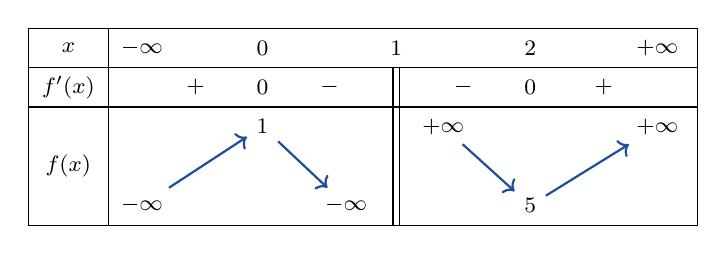
\begin{tikzpicture}[x=0.85cm,y=0.5cm,font=\footnotesize]
\draw (0,0) rectangle (10,-5); \draw (0,-1)--(10,-1); \draw (0,-2)--(10,-2); \draw (1.2,0)--(1.2,-5);
\draw (5.45,-1)--(5.45,-5); \draw (5.55,-1)--(5.55,-5);
\node at (0.6,-0.5){$x$}; \node at (0.6,-1.5){$f^{\prime}(x)$}; \node at (0.6,-3.5){$f(x)$};
\node at (1.7,-0.5){$-\infty$}; \node at (3.5,-0.5){$0$}; \node at (5.5,-0.5){$1$}; \node at (7.5,-0.5){$2$}; \node at (9.4,-0.5){$+\infty$};
\node at (2.5,-1.5){$+$}; \node at (3.5,-1.5){$0$}; \node at (4.5,-1.5){$-$}; \node at (6.5,-1.5){$-$}; \node at (7.5,-1.5){$0$}; \node at (8.6,-1.5){$+$};
\node (m) at (1.7,-4.5){$-\infty$}; \node (a) at (3.5,-2.5){$1$}; \node (b) at (4.75,-4.5){$-\infty$};
\node (c) at (6.2,-2.5){$+\infty$}; \node (d) at (7.5,-4.5){$5$}; \node (p) at (9.4,-2.5){$+\infty$};
\draw[->,cDef,thick] (m)--(a); \draw[->,cDef,thick] (a)--(b); \draw[->,cDef,thick] (c)--(d); \draw[->,cDef,thick] (d)--(p);
\end{tikzpicture}\end{LTR}\par المقاربان: $x=1$ و $y=x+2$.\par\smallskip\begin{LTR}\centering \begin{tikzpicture}[x=0.45cm,y=0.3cm,font=\scriptsize]
\draw[->] (-5,0)--(6,0) node[right]{$x$}; \draw[->] (0,-8)--(0,12) node[above]{$y$};
\draw[cThm,dashed] (1,-8)--(1,12) node[right]{$x=1$};
\draw[cRem,dashed,domain=-5:6] plot (\x,{\x+2}); \node[cRem] at (5.2,9.3){$y=x+2$};
\draw[cDef,thick,domain=-5:0.85,samples=60] plot (\x,{\x+2+1/(\x-1)});
\draw[cDef,thick,domain=1.1:5.6,samples=60] plot (\x,{\x+2+1/(\x-1)}); \node[cDef] at (3.6,8){$C_f$};
\end{tikzpicture}\end{LTR}\par }{50 د}{رسم بالحاسبة للتحقق.}
\Row{}{%
\Lab{cThm!80!black}{حذار}\ نرسم المقاربات أولاً ثم المنحني.}{}{}
\Row{التقويم}{%
\Lab{cEx}{تطبيق}\par ادرس الدالة $g(x)=\dfrac{2x+1}{x-1}$: النهايات ، المقاربات ، اتجاه التغير.\par\textbf{الحل:} $g(x)=2+\dfrac3{x-1}$ ؛ $y=2$ و $x=1$ مقاربان ؛ $g^{\prime}(x)=\dfrac{-3}{(x-1)^2}<0$: $g$ متناقصة على كل من المجالين.\par\textbf{واجب منزلي:} تمارين 58 إلى 68 من باب النهايات.\par\smallskip\textbf{ملاحظات حول سير الحصة:} \dotfill}{25 د}{نهاية المحور: فرض أو مراجعة.}
\end{Sayr}
\end{document}
